\appendix

\section{Power loss due to Galactic Binary foreground}
\label{sec:gb_noise_snr_loss}
\updated{As demonstrated in Figure~\ref{fig:psds}, the pre-merger analysis mainly cuts off before the galactic bnary confusion noise becomes significant.}

\updated{Here we calculate how much SNR is lost due to the Galactic Binary confusion noise for each signal.}

\begin{figure}
   \centering
   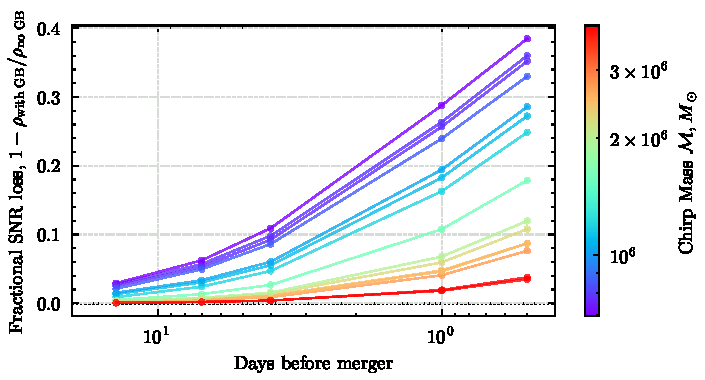
\includegraphics[width=\columnwidth]{images/figure_12_GB_SNR_loss.pdf}
   \caption{
       \updated{Fractional signal-to-noise ratio loss for each signal caused by Galactic Binary confusion noise.
       We see that signals at lower chirp masses are affected more, losing up to 39\% of power half a day before merger.
       For heavier signals, and for times more than a few days before merger, the signal power loss is much less, below 10\%.}
   }
   \label{fig:removal_residual}
\end{figure}

\section{Signal Removal}
\label{sec:signal_removal}
\updated{As discussed in Section~\ref{sec:focused}, the loudest signals from the data can match to templates in the bank even with the small amount of template power away from the merger.
The solution is to manually remove signals from the data as soon as they are known.
This is similar to the global fit challenge, but remains within the same source type.
To remove signals from the data, we assume that the signal is known perfectly, and the parameters of the injection are use to generate a waveform which is subtracted from the data.}

\updated{As shown in Figure~\ref{fig:removal_residual}, signal removal is not perfect, and some signal power remains.
We encourage the release of the exact methods which were used to produce the datasets so that they can be independently recreated.}

\begin{figure}
   \centering
   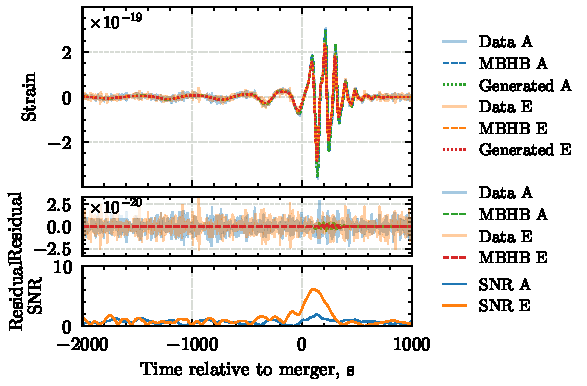
\includegraphics[width=\columnwidth]{images/figure_11_removal_residual.pdf}
   \caption{
       \updated{Residuals after removal for Signal 3.
       Equivalent plots for all signals are included in the data release.}
   }
   \label{fig:removal_residual}
\end{figure}

\updated{The remaining signal power still produces a small signal-to-noise ratio peak, as in Figure~\ref{fig:variable_removal}.
Early estimate parameter estimation routines may find parameters which remove more of the signal from the data, and so this may not be an issue in real LISA premerger analyses.}